\documentclass[11pt,a4paper]{article}
\usepackage[margin=23mm]{geometry}
\usepackage[T1]{fontenc}
\usepackage{lmodern,microtype,amsmath,amssymb,booktabs,tabularx,array}
\usepackage{tikz,pgfplots}
\usetikzlibrary{arrows.meta,positioning}
\pgfplotsset{compat=1.18}
\usepackage{caption,placeins,xurl}
\usepackage[colorlinks=true,linkcolor=blue!45!black,citecolor=blue!45!black,urlcolor=blue!45!black]{hyperref}
\hypersetup{pdftitle={Application-Aware Handoffs in Dense Wireless Networks},pdfauthor={Mouhamad Mamane}}
\setlength{\parskip}{4pt}
\setlength{\parindent}{0pt}
\setlength{\emergencystretch}{2em}
\captionsetup{font=small,labelfont=bf}
\newcommand{\code}[1]{\texttt{\small #1}}
\newcommand{\pp}{\,\text{percentage points}}
\title{Application-Aware Handoffs in Dense Wireless Networks\\[5pt]\large A Packet-Queue Simulation Study}
\author{Mouhamad Mamane\\\normalsize\href{mailto:mmm466@case.edu}{mmm466@case.edu}}
\date{14 October 2026}
\begin{document}
\maketitle
\begin{abstract}
A moving Wi-Fi device may see a stronger access point while its current connection still supports a call. Changing access points can improve capacity, but scanning, transition delay, and queue loss can also interrupt real-time traffic. This study tests a simple application-aware handoff rule that combines estimated capacity, queue delay, signal trend, transition cost, report age, and recent missed deadlines. A reproducible packet-queue model generates simultaneous voice packets and packetized video frames, while fixed background users compete for airtime. The main test contains ten policies, six environments, and forty paired seeds, giving 2,400 policy runs. The primary measure is the equally weighted mean of voice-packet and video-frame deadline-miss fractions. The proposed rule scores 2.047\%, compared with 1.943\% for a separately tuned application-margin rule. Its paired difference is +0.104 percentage points, with a 95\% seed-block bootstrap interval of [0.038, 0.173]. A simpler capacity-and-load rule has the lowest overall score, 1.282\%, but loses to other rules in some environments. Eight sensitivity checks expose further limits, including strong effects of degraded reports and numerical time step. The results support careful baseline tuning and direct accounting of missed deadlines. They do not establish interruption-free roaming or performance on real Wi-Fi hardware.
\end{abstract}
\noindent\textbf{Keywords:} Wi-Fi roaming; access-point selection; real-time traffic; deadline misses; simulation; reproducibility.

\section{Introduction}
A person walking across a campus may pass several Wi-Fi access points (APs) during a voice or video call. The strongest signal is useful information, but it does not describe the full connection. A nearby AP may be busy. A move to a better AP may also take time, fail, or lose queued data. A useful roaming rule must balance the expected gain against the disruption caused by the move.

IEEE 802.11k, 802.11v, and 802.11r support neighbor information, transition assistance, and faster transitions. Client behavior still matters. Vendor documentation also shows that real clients can consider factors beyond signal strength, including load~\cite{M01}. Therefore, a strongest-signal rule is a simple experimental baseline; it is not a complete model of every commercial device.

The practical goal is to protect real-time applications during roaming. Here, we ask a narrower question that can be tested: \emph{under declared traffic, observation, and transition assumptions, does an application-aware rule with added caution and a short signal-trend estimate reduce missed delivery deadlines compared with a tuned fixed-margin rule?} We also ask how the answer changes with load, movement, stale reports, transition cost, and simulation resolution.

This paper provides three contributions. First, it gives a transparent packet-queue model with finite buffers, whole-frame delivery checks, delayed information, and competition with background users. Second, it develops and tunes a handoff rule and compares it with simple policies and four component removals. Third, it reports the complete evaluation, including negative results, uncertainty intervals, sensitivity checks, and reproducible data. The work does not claim that application-aware roaming is a new idea or that the proposed rule is a universal improvement.

The main result is unfavorable to the proposed rule. It has more missed deadlines and more handoff attempts than the tuned application-margin baseline. The simpler capacity-and-load rule performs best on the declared average, although it is not best in every environment. This result is useful because fewer or more carefully scored handoffs do not automatically produce better application delivery.

\section{Related work and research position}
Application-aware AP selection has an established history. Kim et al. studied selection based on user applications in dense WLANs~\cite{F01}. Dely et al. included handover costs in WLAN association optimization~\cite{F02}. Adame et al. studied channel-load-aware AP and extender selection using IEEE 802.11k/v~\cite{F03}. These works motivate the use of application demand, network load, and switching cost. The present rules are independently specified heuristics, not reproductions of those algorithms.

Recent work explores several different approaches. Wong and Tan proposed a load-aware handover method for dense 802.11 networks~\cite{R03}. Wang et al. investigated distributed multi-agent deep Q-learning for fast roaming~\cite{R06}. Lee et al. explored on-device language models for context-aware Wi-Fi roaming~\cite{R04}. Kwon et al. used LSTM prediction in industrial Wi-Fi mobility~\cite{R13}. Prediction accuracy and roaming performance are different outcomes: predicting a transition does not by itself show that delivered media improves after taking that action.

Other work changes the transition mechanism or hardware. Scanzio et al. considered multi-link operation and wireless digital twins for enhanced roaming~\cite{R07}. Avila-Campos et al. studied mobility for Wi-Fi-based time-sensitive networks~\cite{M06}. Such designs have different capabilities from the single-link client modeled here. Their results are not used to calibrate the transition distribution in this study.

Two 2026 sources are particularly close to the broad motivation. Sueda et al. describe handover control based on application context~\cite{R01}; Nadeem et al. describe a QoS-aware framework for software-defined Wi-Fi~\cite{R02}. Only their abstracts, metadata, or indexed excerpts were available in this review. Their full methods were not inspected. This limits any claim about novelty or direct superiority over the latest work.

The targeted review, with a cutoff of 14 October 2026, records 21 research works and 13 technical or author-guidance documents. Fourteen research works were inspected through selected full-text passages and seven at abstract or excerpt depth. Sixteen research works date from 2023--2026. The review is not a systematic search of every database, and no external algorithm was independently reproduced. The repository records the access depth and verified source information for each entry.

For real-time traffic, late delivery can have little use even when throughput is high~\cite{P01}. RFC 7587 provides a 20 ms default packetization time for Opus~\cite{P02}; this supports a plausible voice timing choice, not a universal network deadline. The deadlines in this paper are explicit research assumptions. Likewise, our missed-frame-run measure is not the decoded-video freeze statistic defined by W3C WebRTC statistics~\cite{M12}.

\section{System model}
\subsection{Scope and network structure}
The simulator represents one moving client with simultaneous voice and video traffic. Each AP also serves fixed background users. All APs are on the same subnet. Each AP has a separate airtime budget and shares it among its active users. When the moving client changes AP, the service available to background users can change. Background users keep their associations. Their offered rates follow the declared external load patterns and do not adapt to congestion.

This is a packet-queue abstraction, not an IEEE 802.11 MAC or full network stack. It omits contention windows, collisions, retransmissions, channel interference between APs, authentication exchanges, backhaul limits, and IP address changes. Dense conditions mean nearby APs and competition within each AP here. They do not cover every effect of a dense wireless deployment. Figure~\ref{fig:model} shows the modeled information path.

\begin{figure}[htbp]
\centering
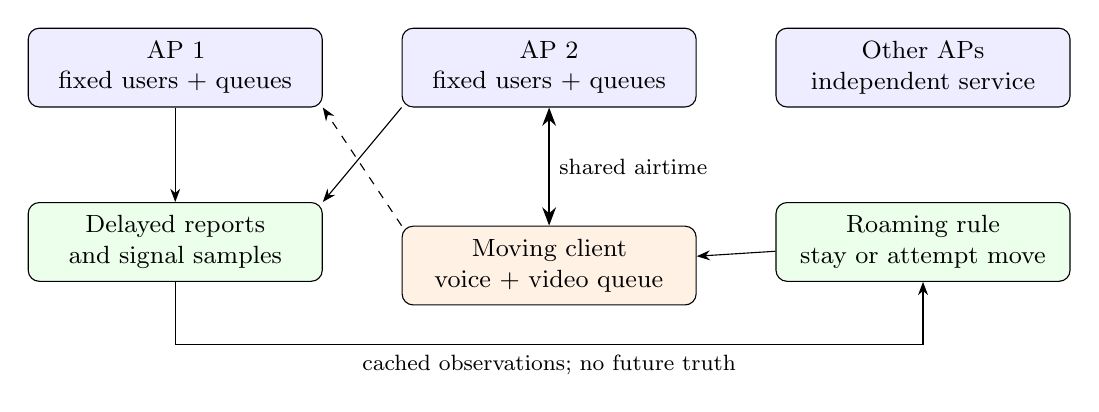
\begin{tikzpicture}[>=Stealth,font=\small,box/.style={draw,rounded corners,align=center,minimum height=10mm,text width=35mm},node distance=8mm and 10mm]
\node[box,fill=blue!7] (ap1) {AP 1\\fixed users + queues};
\node[box,fill=blue!7,right=of ap1] (ap2) {AP 2\\fixed users + queues};
\node[box,fill=blue!7,right=of ap2] (ap3) {Other APs\\independent service};
\node[box,fill=orange!10,below=15mm of ap2] (mobile) {Moving client\\voice + video queue};
\node[box,fill=green!8,below=12mm of ap1] (obs) {Delayed reports\\and signal samples};
\node[box,fill=green!8,below=12mm of ap3] (rule) {Roaming rule\\stay or attempt move};
\draw[<->,thick] (ap2)--node[right,font=\footnotesize]{shared airtime}(mobile);
\draw[->] (ap1)--(obs);\draw[->] (ap2.south west)--(obs.north east);
\draw[->] (obs.south)--++(0,-8mm)-|node[pos=.25,below,font=\footnotesize]{cached observations; no future truth}(rule.south);
\draw[->] (rule)--(mobile);\draw[dashed,->] (mobile.north west)--(ap1.south east);
\end{tikzpicture}
\caption{Model structure, not a measured campus map. Only one client roams. An attempted move interrupts its service and may fail. AP reports contain assumed telemetry richer than ordinary signal readings. The model has no interference between APs.}\label{fig:model}
\end{figure}

\subsection{Time, movement, and link service}
Traffic generation lasts 60 s. The default service step is 10 ms, followed by a drain period of at least 0.3 s. The drain is also required to exceed the larger deadline by one step. Thus, the last generated objects remain in the outcome denominator and have time to reach their deadlines. Voice and video use their own creation clocks. An object created between service steps enters at the next step but keeps its original timestamp. Report sampling, report delivery, and expiry checks are processed at service boundaries. Changing the step therefore changes observation timing as well as service interpolation.

External radio noise and background arrivals use a fixed 20 ms grid. This grid does not change in the 5 ms and 20 ms service-step checks. Separate random streams generate signal noise, background traffic, report errors, handoff outcomes, and frame sizes. Every policy in a scenario--seed pair uses the same external world. Transition draws are indexed by decision time and target AP, so an extra action by one policy does not consume another policy's future random values.

The route runs 3 m to the side of the AP line. At distance $d_i$ metres, the signal and assumed link rate are
\begin{align}
 s_i &= -36-30\log_{10}(d_i)+\epsilon_i \quad\text{dBm},\\
 R(s_i)&=\begin{cases}0,&s_i<-85,\\\min\{54,54\,10^{(s_i+55)/20}\},&s_i\geq-85,\end{cases}\quad\text{Mb/s}.
\end{align}
The Gaussian noise has a 0.4 s correlation time and a scenario-specific standard deviation. Background links have a fixed rate of 54 Mb/s. These smooth curves and thresholds are assumed values, not calibrated radio measurements or actual modulation choices.

Within each step, nonempty users share AP airtime equally. Unused shares are redistributed. The moving client joins this sharing only while its radio is active. Packet completion times are interpolated over its active part of the step. This is fluid sharing rather than a sequence of real transmissions. A short isolated packet can be credited at the end of the step; reported simulated delay therefore depends partly on the numerical resolution.

\subsection{Traffic and queues}
Table~\ref{tab:settings} gives the main settings. A voice packet succeeds only when all its bytes arrive by its deadline. A video frame is split into fragments and succeeds only when every fragment arrives by the frame deadline. Video frame sizes are independent uniform draws between 75\% and 125\% of the nominal size. Frames have no codec dependencies, concealment, feedback, or adaptive bitrate.

\begin{table}[htbp]\centering\small
\caption{Main assumptions. These values define the experiment; they are not measurements or mandatory application standards.}\label{tab:settings}
\begin{tabularx}{\linewidth}{@{}lX@{}}\toprule
Quantity & Value or rule \\ \midrule
Voice & 160 bytes every 20 ms; deadline 60 ms (64 kb/s)\\
Video & 30 frames/s; mean 2.4 Mb/s; deadline 150 ms\\
Video fragments & At most 1,200 bytes; all fragments needed\\
Moving-client queue & 256 packets; earliest-deadline-first service\\
Background queues & 256 packets/user; 1,200-byte packets; FIFO\\
Scan & Every 1 s; 12 ms service interruption\\
Signal samples & Serving sample every 100 ms; 40 ms report delay\\
AP reports & Every 500 ms, asynchronous; delay $300\pm150$ ms\\
Load measurement & Background-airtime average, 0.5 s time constant; noise SD 0.05\\
Transition & Uniform 40--120 ms; failure probability 0.03\\
Failed transition & Additional 120 ms; return to old AP\\
Queued data at attempt & Discard old moving-client queue; retain new arrivals\\
Attempt interval / emergency & Normally 1 s / cached serving signal below $-78$ dBm\\\bottomrule
\end{tabularx}
\end{table}

The moving client's queue uses earliest-deadline-first service for every policy. Overflow, expiry, and handoff losses remain in the miss denominator. A packet completed exactly at its deadline is on time. A packet completed late counts toward delivered bytes but not on-time bytes. An expired partial packet consumes service without counting as a completed delivery.

Each background user receives synthetic packet batches every 20 ms. Counts use Poisson draws for means below ten packets and a rounded normal approximation otherwise. Offered background load is a fraction of nominal AP capacity and can exceed one. Flat, unequal, alternating, and bursty patterns create different queue conditions. These are fixed-rate sources, not TCP flows. Equal-size background packets are stored as exact counts and partial-head bytes; foreground packets are represented individually.

\subsection{Observations and action costs}
Decisions occur every 100 ms, and no new attempt starts while a transition is pending. Serving-signal and own-miss sampling continue on this clock during scans and transitions. This is an idealized measurement assumption. Every policy starts on the strongest AP using one free initial signal snapshot, with a common initial load estimate of 0.5. After startup, all policies pay the same periodic scanning cost. Candidate signal samples become available after the scan and report delay. Serving signal is also delayed. Reports retain their source timestamps, and an older report cannot replace a newer one.

AP telemetry contains background-airtime use, the number of active background queues, and total queued background bytes converted to a delay estimate at 54 Mb/s. All fields are delayed. Only background-airtime load has added measurement noise; active-user count and queue delay are exact source-state values before delay. The serving AP has no privileged fresh queue report. These quantities require an assumed telemetry service. They are not all supplied automatically by IEEE 802.11k/v, and their transport overhead is not modeled.

The client also receives a delayed estimate of its own recent misses. It counts voice-packet and video-frame deadlines that already elapsed in the preceding second. Future and pending deadlines cannot enter this estimate. Own-miss reports are sampled every 100 ms and delayed by a fixed 300 ms without jitter (1.5 s in the stale-report condition). Each media unit has one vote here; this differs from the equal stream weights of the primary outcome.

A scan or transition prevents focal service for its actual duration, including fractional steps. Background users can use that airtime. Overlapping scan and transition intervals are counted by their union. A failed transition returns to the old AP after the additional delay. The default queue flush at an attempt is a strong assumption and is tested separately with queue retention. New packets generated during a blackout can wait in the queue. No modeled controller knows the realized duration of its next transition.

\section{Handoff rules}
\subsection{Shared estimates and simple policies}
Let $\hat s_i$ be cached signal, $\hat b_i$ reported background airtime, $\hat n_i$ active background users, and $\hat q_i$ estimated queue delay at AP $i$. The estimated capacity and application score are
\begin{align}
 \hat C_i &=R(\hat s_i)\max\left(1-\hat b_i,\frac{1}{\hat n_i+1}\right),\label{eq:capacity}\\
 U_i &=\min\left(1,\frac{\hat C_i}{D}\right)\max\left(0,1-\frac{\hat q_i}{2B}\right),\label{eq:utility}
\end{align}
where $D=2.464$ Mb/s is nominal combined demand and $B$ is the smaller application deadline. The capacity estimate combines unused airtime with a fair-share floor. The controller uses the same assumed signal-to-rate curve as the service model. Delayed observations still create error, but the rate calibration itself is correctly specified by construction.

The \emph{Signal} rule selects stronger cached signal with a tuned dB margin. \emph{Capacity/load} selects higher $\hat C_i$ with a tuned relative margin. \emph{App margin} selects higher $U_i$ with a tuned absolute margin. \emph{Session stay} remains on its AP unless the common signal emergency occurs. \emph{Earlier caution} adds transition-cost and age terms over a fixed planning horizon, adapting the earlier experiment's idea. Its selected horizon is 16 s, cost weight is 1, age weight is 0.08, and margin is 0.05. It has no own-miss guard; its cost and age penalties remain even during a signal emergency. These are stylized baseline families, not named commercial clients or exact published implementations.

All rules normally require one second since the previous handoff attempt, including a failed attempt. There is no initial waiting period. A cached serving signal below $-78$ dBm removes this restriction and the ordinary improvement margin. Policies share the observation-generation rules, but their reports can differ after their actions change queues. Equal access to information does not mean identical action-dependent observations.

\subsection{Proposed rule}
The proposed rule adds a signal-trend holding estimate and a delayed-miss guard. For a candidate with recent slope $\dot s_i<-0.15$ dB/s,
\begin{equation}
 H_i=\operatorname{clip}\left(\frac{\hat s_i+78}{-\dot s_i},0.25,3\right)\ \text{s};
\end{equation}
otherwise $H_i=3$ s. The slope uses two received samples and their source times. It is a rough linear estimate, not a learned predictor or knowledge of the future route.

Expected switching cost is $\hat c=\beta\bar t+p_f t_f$, where $\bar t$ is mean transition duration, $p_f$ is failure probability, $t_f$ is extra failure delay, and $\beta$ is the controller's cost-belief factor. Normally $\beta=1$. With $a_i$ the larger of signal age and load-report age in seconds, a candidate has adjusted score
\begin{equation}
 V_i=U_i\max\left(0,1-\frac{w_c\hat c}{H_i}\right)-w_a\frac{a_i}{a_i+1\ \text{s}}.\label{eq:adjusted}
\end{equation}
The serving AP retains its unadjusted $U$. The candidate must exceed it by the configured margin. Report age is a caution penalty, not a calibrated probability or confidence interval.

The guard activates if cached serving signal is below $-78$ dBm or the delayed own-miss fraction exceeds 0.25. It bypasses residence, cost, age, and margin restrictions, then chooses an alternative only if its raw $U$ improves on the serving score. This is a recovery attempt based on old information, not a guarantee of recovery. The normal proposed margin is 0.05; development selects $w_c=2$ and $w_a=0.02$.

The decision sequence is: update only received observations; check the guard and residence rule; compute each candidate's raw score; apply trend, cost, and age terms when the guard is inactive; select the highest eligible alternative; and attempt a move only if the required improvement exists. The score guides decisions, while delivered packet and frame deadlines determine outcomes independently.

Four removals test the local role of each component. \emph{No dwell} uses a fixed horizon. \emph{No guard} removes the additional recovery rule but keeps the common signal emergency. \emph{No cost} removes the cost discount. \emph{No age} removes the age penalty. Each keeps the other selected parameters and is not retuned.

\section{Experiment design and analysis}
\subsection{Development and frozen evaluation}
Three development environments use 24 m AP spacing with corridor, unequal-load, and reversing movement patterns. Seeds 20001--20008 give 24 development worlds. An initial search contains 19 settings and 456 policy executions. Several selected values lie at search boundaries, and the proposed method loses to simpler rules in development. One documented extension therefore tests 43 settings, giving another 1,032 executions on the same worlds. The first search and its protocol remain archived.

The final grid tests four Signal margins (0, 1, 3, 5 dB), five Capacity/load margins (0.05, 0.15, 0.30, 0.50, 0.75), six App margins (0, 0.03, 0.08, 0.15, 0.25, 0.40), and four Earlier caution horizons (1, 3, 8, 16 s). The proposed family tests 24 combinations: cost weights $\{0.5,1,2,4\}$, age weights $\{0,0.02\}$, and guard thresholds $\{0.02,0.10,0.25\}$. Its search budget is larger than each baseline's budget.

Selection minimizes the equally weighted development deadline-miss score, breaking ties by fewer handoffs and then variant identifier. Selected baseline settings are Signal 1 dB, Capacity/load 0.75, App margin 0.15, and Earlier caution 16 s. The last two boundary selections for Capacity/load and Earlier caution are reported without another search extension. These are tested grid choices, not globally optimal parameters.

Code, protocol, and chosen settings are locally frozen before held-out evaluation. This is not external preregistration. The one grid extension is explicitly development-informed. No held-out outcome selects parameters or triggers another model revision. Table~\ref{tab:scenarios} describes the final environments. Each has 40 seeds, 50001--50040, and all ten policies: 240 paired worlds and 2,400 policy runs. A straight path stops at its endpoint; a sinusoidal path's stated speed is its maximum.

\begin{table}[htbp]\centering\small
\caption{Held-out environment definitions. Load is nominal background demand relative to 54 Mb/s before pattern multipliers. All but Crowded have four fixed users/AP and 2 dB signal-noise SD. Crowded has twelve users/AP and 2.5 dB SD.}\label{tab:scenarios}
\begin{tabularx}{\linewidth}{@{}lXlll@{}}\toprule
Environment & AP positions (m) & Movement & Speed (m/s) & Load\\\midrule
Wide corridor & 0,30,60,90,120,150 & Linear & 1.8 & 0.40 flat\\
Short cells & 0,12,24,36,48,60 & Shuttle & 4.5 & 0.50 alternate\\
Reversals & 0,19,38,57,76,95 & Shuttle & 2.6 & 0.60 alternate\\
Hidden hotspot & 0,17,42,68,92,122 & Linear & 2.3 & Unequal\\
Burst load & 0,21,44,67,91,116 & Linear & 2.0 & 0.48 bursts\\
Crowded & 0,17,34,51,68,85,102,119 & Sine & 1.5 & 0.85 bursts\\\bottomrule
\end{tabularx}
\end{table}

The hidden-hotspot base loads are 0.25, 0.90, 0.30, 0.85, 0.45, and 0.70. Alternating patterns multiply odd-indexed AP loads by 1.35 and even-indexed loads by 0.45. Bursts move a high-load group between APs using multipliers 1.65 and 0.45, with periods of 5 s for Burst load and 4 s for Crowded. Offered load is bounded at 1.5. Exact routes and remaining settings are stored in the configuration.

\subsection{Outcomes and uncertainty}
For every run, the primary score is
\begin{equation}
 M=\frac12\frac{N_{\mathrm{voice,miss}}}{N_{\mathrm{voice}}}+\frac12\frac{N_{\mathrm{frame,miss}}}{N_{\mathrm{frame}}}.
\end{equation}
Every offered object counts, including traffic lost to overflow, expiry, a handoff, or a deadline during a blackout. Main runs generate 3,000 voice packets and 1,800 video frames. Equal stream weights are an engineering choice, so both components are also shown separately. A frame with one missing fragment fails even if its other fragments arrive.

Interruption measures use consecutive missed scheduled media units. The longest voice miss run is its slot count times 20 ms; the video measure is its frame count divided by 30. A video long-run fraction counts all frames in maximal miss runs of at least six frames, about 200 ms. This includes the first five frames when a run qualifies. These are scheduled-deadline proxies, not recorded sound gaps, decoder freezes, or the W3C freeze definition~\cite{M12}.

Other outcomes are handoff attempts and failures, on-time delivered bytes, delay among completed packets, and background delivery. The delay statistic excludes packets that never complete and must be read beside the miss rate. Within-run packet-delay p95 uses nearest rank, $\lceil0.95n\rceil$; cross-run percentiles and bootstrap endpoints use linear interpolation. Background delivery covers the simulation and drain period. Its worst-user measure is the lowest delivered/offered ratio among users with offered traffic.

The primary comparison is Proposed minus App margin. For each seed, we average its six paired scenario differences, then bootstrap these 40 seed blocks with 5,000 resamples and analysis seed 81631. We report a percentile 95\% interval. Negative differences favor Proposed. This preserves pairing and avoids treating packets as independent trials. The average describes the declared equal mix of six environments. Scenario-specific and secondary intervals are descriptive and unadjusted for multiple comparisons. They quantify stochastic uncertainty inside the model, not uncertainty about real hardware or omitted mechanisms.

\subsection{Sensitivity checks and trace selection}
Eight conditions use the same four environments (Short cells, Hidden hotspot, Burst load, Crowded) and ten seeds (50001--50010). The original plan evaluates Signal, App margin, Earlier caution, and Proposed, giving 1,280 runs. A separate supplement adds Capacity/load to all eight conditions, giving 320 runs. Its specification was frozen after development and before held-out outcomes were inspected. It is reported as a secondary extension, not part of the initial sensitivity protocol. No condition retunes the selected parameters.

The changes are: deadlines of 40/100 ms or 100/250 ms for voice/video; costly transitions with mean 180 ms, half-width 80 ms, failure probability 0.10, extra failure delay 250 ms, and a 40 ms scan; stale reports every 1 s with delay $1.5\pm0.4$ s and load-noise SD 0.12; cost belief $\beta=0.25$; service steps of 5 or 20 ms; and retention of queued focal packets during handoff. The cost-belief change scales only mean transition duration in the estimate, not expected failure-extra cost. Other changes are known to the controller through the test configuration.

The matched reference uses the same four environments and ten seeds from the main data. It is a subset, not new experiments. The total packet study executes 5,488 policy runs: 456 initial development, 1,032 final development, 2,400 main, 1,280 original sensitivity, and 320 supplementary sensitivity runs. Repeated development settings are not new independent worlds.

Before evaluation, seed 50001 was selected for trace replay in every main environment with Signal, App margin, and Proposed. All 18 replays are checked against their saved main outcomes. The displayed timeline is also selected in advance: Short cells, seed 50001, App margin versus Proposed. It illustrates the mechanism without choosing a favorable example after seeing results.

\section{Results}
\subsection{Main deadline outcomes}
Table~\ref{tab:main} and Figure~\ref{fig:bars} show all ten policies. Proposed has a primary score of 2.047\%, compared with 1.943\% for App margin. The primary paired difference is $+0.104\pp$, with 95\% interval [0.038, 0.173]. Its voice difference is +0.093 percentage points [0.058, 0.131], and its video difference is +0.116 [0.016, 0.220]. The proposed additions therefore do not improve the declared primary outcome.

\begin{table}[htbp]\centering\small
\caption{Main means over 240 worlds per policy. Score, voice misses, and video misses are percentages; handoffs are attempts per 60 s run. Lower miss rates are better.}\label{tab:main}
\begin{tabular}{@{}lrrrr@{}}\toprule
Policy & Score (\%) & Voice (\%) & Video (\%) & Handoffs\\\midrule
% BEGIN GENERATED MAIN_TABLE
Signal & 1.968 & 1.055 & 2.881 & 9.23 \\
Capacity/load & 1.282 & 0.841 & 1.723 & 9.51 \\
App margin & 1.943 & 0.942 & 2.944 & 7.43 \\
Earlier caution & 2.243 & 1.091 & 3.396 & 8.42 \\
Session stay & 7.207 & 2.607 & 11.806 & 5.24 \\
Proposed & 2.047 & 1.035 & 3.059 & 8.63 \\
No dwell & 2.059 & 1.041 & 3.078 & 8.72 \\
No guard & 2.123 & 0.989 & 3.257 & 6.97 \\
No cost & 2.760 & 1.450 & 4.070 & 12.45 \\
No age & 2.068 & 1.049 & 3.087 & 8.74 \\
% END GENERATED MAIN_TABLE
\bottomrule\end{tabular}
\end{table}

\begin{figure}[htbp]\centering
% BEGIN GENERATED BARS
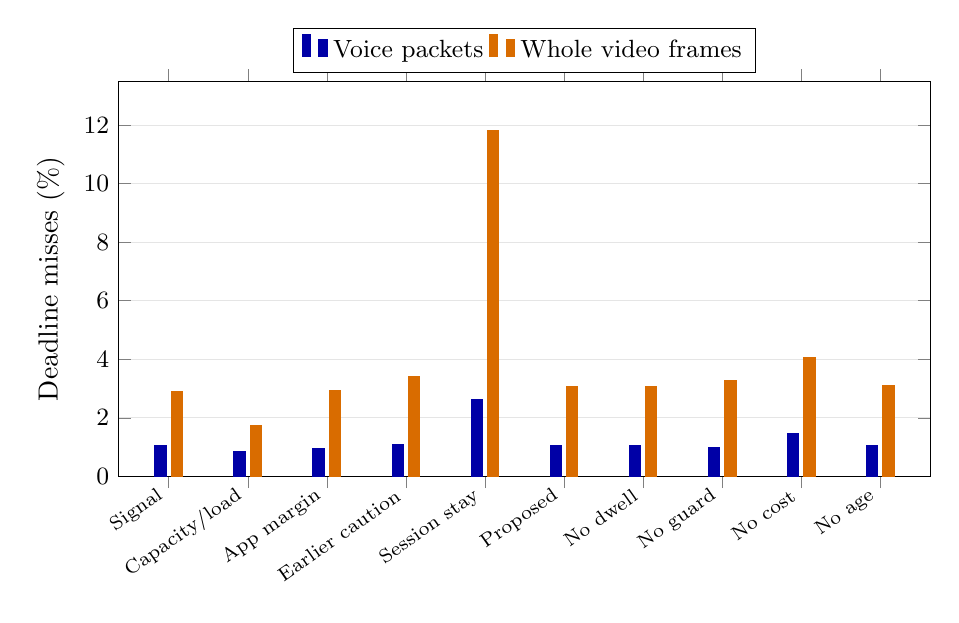
\begin{tikzpicture}
\begin{axis}[width=.98\linewidth,height=66mm,ybar,bar width=4pt,ymin=0,ymax=13.5,
 ylabel={Deadline misses (\%)},xtick={0,...,9},xticklabels={Signal,Capacity/load,App margin,Earlier caution,Session stay,Proposed,No dwell,No guard,No cost,No age},
 x tick label style={rotate=35,anchor=east,font=\scriptsize},tick label style={font=\small},
 enlarge x limits=.07,ymajorgrids,grid style={gray!20},
 legend style={at={(.5,1.02)},anchor=south,legend columns=2,font=\small}]
\addplot[fill=blue!65!black,draw=blue!65!black] coordinates {(0,1.055) (1,0.84125) (2,0.94180556) (3,1.0908333) (4,2.6069444) (5,1.0348611) (6,1.04125) (7,0.98902778) (8,1.4495833) (9,1.0490278)};
\addlegendentry{Voice packets}
\addplot[fill=orange!85!black,draw=orange!85!black] coordinates {(0,2.8810185) (1,1.7229167) (2,2.9435185) (3,3.3958333) (4,11.80625) (5,3.0592593) (6,3.0775463) (7,3.2571759) (8,4.0699074) (9,3.087037)};
\addlegendentry{Whole video frames}
\end{axis}\end{tikzpicture}
% END GENERATED BARS
\caption{Voice-packet and whole-video-frame misses, with every tested policy shown. Each bar is a mean over the same 240 worlds. Voice is the left bar and video the right bar in each pair. This descriptive plot has no uncertainty bars; paired contrasts provide the uncertainty analysis.}\label{fig:bars}
\end{figure}

Capacity/load has the lowest overall score, 1.282\%. Its secondary differences from Signal and App margin are respectively $-0.686\pp$ [\ensuremath{-}0.776, \ensuremath{-}0.594] and $-0.661\pp$ [\ensuremath{-}0.752, \ensuremath{-}0.573]. Proposed is worse than Capacity/load by $+0.765\pp$ [0.668, 0.865]. These comparisons support the simpler rule within this model and mix of environments; they do not prove it is best on arbitrary networks.

Session stay has the fewest average attempts, 5.24, but the highest deadline score, 7.207\%. Proposed makes 8.63 attempts, compared with 7.43 for App margin. Their paired difference is +1.20 attempts [0.93, 1.48]. Thus, the proposed rule also makes more handoff attempts than App margin in this packet study. Capacity/load makes 9.51 attempts while obtaining fewer misses. Handoff count alone is an incomplete measure of quality.

\subsection{Differences between environments}
Figure~\ref{fig:scenario} reports Proposed minus App margin by environment. The Crowded result is an important source of the overall loss. Its proposed score is 6.224\%, compared with 5.820\% for App margin. Burst load is almost tied at 2.526\% and 2.527\%. Near-zero point differences must not be presented as firm wins.

\begin{figure}[htbp]\centering
% BEGIN GENERATED SCENARIO
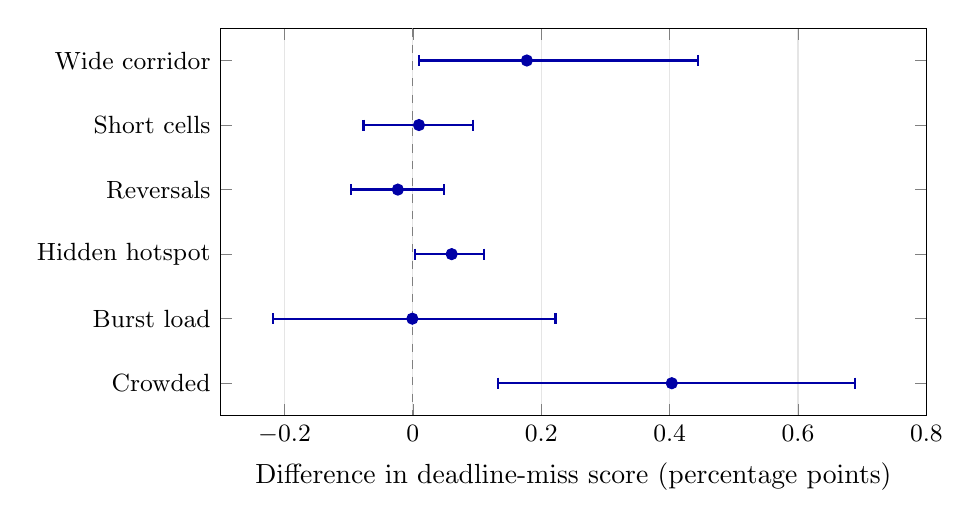
\begin{tikzpicture}\begin{axis}[width=.87\linewidth,height=65mm,
 xlabel={Difference in deadline-miss score (percentage points)},ytick={0,...,5},
 yticklabels={Wide corridor,Short cells,Reversals,Hidden hotspot,Burst load,Crowded},y dir=reverse,ymin=-.5,ymax=5.5,
 xmin=-.3,xmax=.8,xmajorgrids,grid style={gray!20},tick label style={font=\small}]
\addplot[gray,dashed] coordinates {(0,-.5)(0,5.5)};
\addplot[blue!65!black,thick,mark=|] coordinates {(0.0093055556,0) (0.44376042,0)};
\addplot[blue!65!black,only marks,mark=*] coordinates {(0.1775,0)};
\addplot[blue!65!black,thick,mark=|] coordinates {(-0.0768125,1) (0.094170139,1)};
\addplot[blue!65!black,only marks,mark=*] coordinates {(0.0094444444,1)};
\addplot[blue!65!black,thick,mark=|] coordinates {(-0.096805556,2) (0.048614583,2)};
\addplot[blue!65!black,only marks,mark=*] coordinates {(-0.023472222,2)};
\addplot[blue!65!black,thick,mark=|] coordinates {(0.00375,3) (0.11083333,3)};
\addplot[blue!65!black,only marks,mark=*] coordinates {(0.060416667,3)};
\addplot[blue!65!black,thick,mark=|] coordinates {(-0.21778125,4) (0.22222569,4)};
\addplot[blue!65!black,only marks,mark=*] coordinates {(-0.00083333333,4)};
\addplot[blue!65!black,thick,mark=|] coordinates {(0.13261806,5) (0.68931944,5)};
\addplot[blue!65!black,only marks,mark=*] coordinates {(0.40333333,5)};
\end{axis}\end{tikzpicture}
% END GENERATED SCENARIO
\caption{Proposed minus App margin in the primary score. Positive values favor App margin. Intervals are paired 95\% bootstrap intervals within each environment, based on 40 pairs, without adjustment for multiple comparisons. The dashed line marks equal performance.}\label{fig:scenario}
\end{figure}

Capacity/load also has clear exceptions. In Burst load, its score is 0.765\%, compared with 0.481\% for Signal, a difference of +0.284 percentage points [0.184, 0.381]. In Short cells, Capacity/load scores 1.330\%, compared with 1.118\% for App margin, a difference of +0.211 [0.073, 0.350]. Fast load changes and short residence opportunities can challenge a delayed capacity estimate. This explanation is consistent with the model, but the aggregate comparison alone does not isolate a unique cause.

\subsection{Interruption lengths and other users}
The mean of each run's longest voice miss run is 101.2 ms for Proposed, 96.8 ms for App margin, and 89.3 ms for Capacity/load. Across the 240 run maxima, their 95th percentiles are 220, 201, and 180 ms. Figure~\ref{fig:cdf} shows the distribution rather than hiding these tails behind one average.

\begin{figure}[htbp]\centering
% BEGIN GENERATED CDF
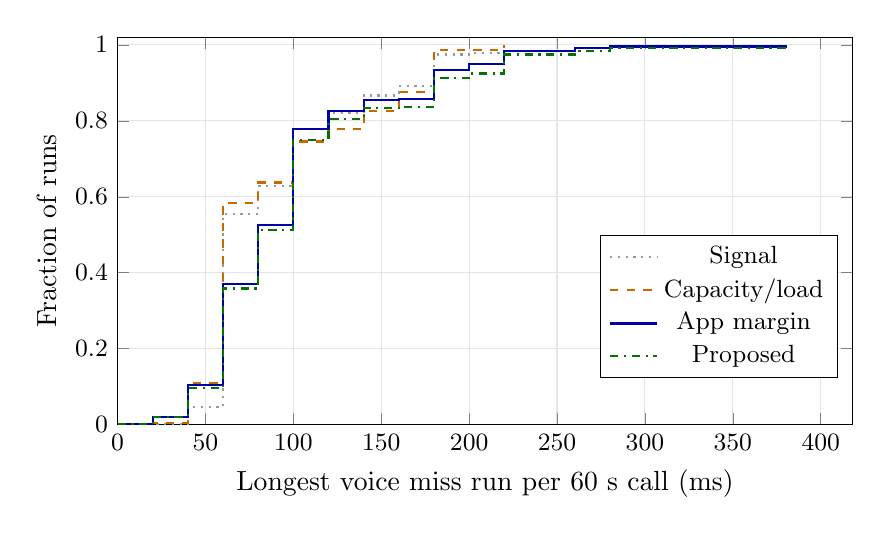
\begin{tikzpicture}\begin{axis}[width=.90\linewidth,height=65mm,
 xlabel={Longest voice miss run per 60 s call (ms)},ylabel={Fraction of runs},
 ymin=0,ymax=1.02,xmin=0,xmajorgrids,ymajorgrids,grid style={gray!20},
 legend style={at={(.98,.12)},anchor=south east,font=\small},tick label style={font=\small}]
\addplot[const plot,thick,gray!80,dotted] coordinates {(0,0) (40,0.045833333) (60,0.55416667) (80,0.62916667) (100,0.77916667) (120,0.82083333) (140,0.86666667) (160,0.89166667) (180,0.975) (200,0.97916667) (220,1)};
\addlegendentry{Signal}
\addplot[const plot,thick,orange!80!black,dashed] coordinates {(0,0) (20,0.0041666667) (40,0.10833333) (60,0.58333333) (80,0.6375) (100,0.74583333) (120,0.77916667) (140,0.825) (160,0.875) (180,0.9875) (220,1)};
\addlegendentry{Capacity/load}
\addplot[const plot,thick,blue!65!black,solid] coordinates {(0,0) (20,0.020833333) (40,0.10416667) (60,0.37083333) (80,0.525) (100,0.77916667) (120,0.825) (140,0.85416667) (160,0.85833333) (180,0.93333333) (200,0.95) (220,0.98333333) (260,0.99166667) (280,0.99583333) (380,1)};
\addlegendentry{App margin}
\addplot[const plot,thick,green!45!black,dashdotted] coordinates {(0,0) (20,0.020833333) (40,0.095833333) (60,0.35833333) (80,0.5125) (100,0.75) (120,0.80416667) (140,0.83333333) (160,0.8375) (180,0.9125) (200,0.925) (220,0.975) (260,0.98333333) (280,0.99166667) (380,1)};
\addlegendentry{Proposed}
\end{axis}\end{tikzpicture}
% END GENERATED CDF
\caption{Empirical distribution of the longest voice miss run in each main run, with 240 values per policy. At a fixed duration, a higher curve means more runs remain at or below that duration. The metric concerns scheduled packet deadlines, not heard audio. Tied durations are counted together.}\label{fig:cdf}
\end{figure}

There is one useful but limited tradeoff against App margin. Proposed reduces the mean longest video miss run from 482.1 to 458.8 ms, a paired difference of $-23.3$ ms [\ensuremath{-}41.4, \ensuremath{-}4.4]. Yet it misses more video frames overall. Its video long-run fraction is 2.211\%, compared with 2.185\%; the paired difference of +0.026 percentage points has interval [\ensuremath{-}0.066, 0.118]. A shorter maximum miss run does not establish better overall video quality.

Mean on-time delivery is 2.406 Mb/s for Proposed, 2.409 Mb/s for App margin, and 2.429 Mb/s for Capacity/load. The mean run-level 95th-percentile delay among completed packets is 1.34 ms higher for Proposed than for App margin [0.55, 2.17]. This conditional delay statistic cannot account for packets that never arrived.

Background aggregate delivery is 96.223\% for Proposed, 96.222\% for App margin, and 96.153\% for Capacity/load. Their mean worst-user ratios are 94.587\%, 94.583\%, and 94.480\%. The focal gain of Capacity/load therefore comes with a small lower background delivery ratio in this experiment. These fixed-user summaries are not a general fairness guarantee, especially with only one roaming client.

Figure~\ref{fig:timeline} shows the preselected call example. Each colored span marks failed scheduled media units. It helps connect a summary miss rate to interruption patterns, but one run cannot establish an average effect.

\begin{figure}[htbp]\centering
% BEGIN GENERATED TIMELINE
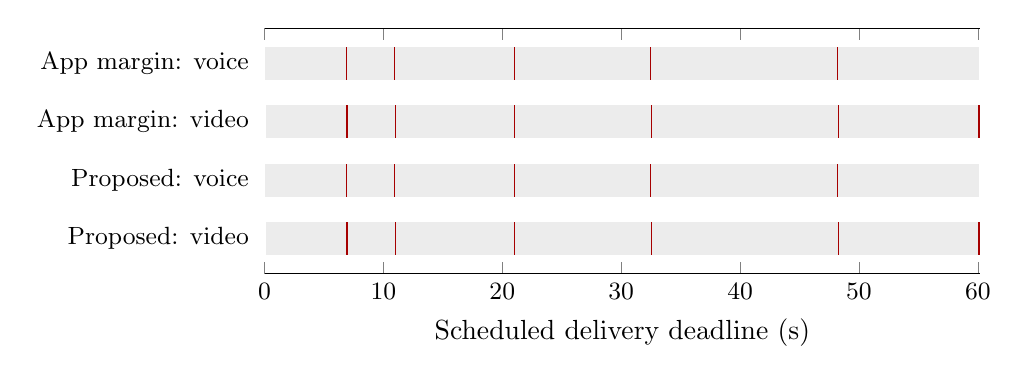
\begin{tikzpicture}\begin{axis}[width=.88\linewidth,height=47mm,
 xmin=0,xmax=60.2,ymin=-.6,ymax=3.6,ytick={3,2,1,0},
 yticklabels={App margin: voice,App margin: video,Proposed: voice,Proposed: video},
 xlabel={Scheduled delivery deadline (s)},tick label style={font=\small},axis y line=left,y axis line style={draw=none},ytick style={draw=none}]
\fill[gray!15] (axis cs:0.06,2.7199999999999998) rectangle (axis cs:60.06,3.2800000000000002);
\fill[red!65!black] (axis cs:6.8600000,2.7199999999999998) rectangle (axis cs:6.9200000,3.2800000000000002);
\fill[red!65!black] (axis cs:10.8600000,2.7199999999999998) rectangle (axis cs:10.8800000,3.2800000000000002);
\fill[red!65!black] (axis cs:20.9600000,2.7199999999999998) rectangle (axis cs:21.0200000,3.2800000000000002);
\fill[red!65!black] (axis cs:32.4600000,2.7199999999999998) rectangle (axis cs:32.4800000,3.2800000000000002);
\fill[red!65!black] (axis cs:48.1600000,2.7199999999999998) rectangle (axis cs:48.1800000,3.2800000000000002);
\fill[gray!15] (axis cs:0.15,1.72) rectangle (axis cs:60.15,2.2800000000000002);
\fill[red!65!black] (axis cs:6.8833333,1.72) rectangle (axis cs:6.9833333,2.2800000000000002);
\fill[red!65!black] (axis cs:10.9500000,1.72) rectangle (axis cs:10.9833333,2.2800000000000002);
\fill[red!65!black] (axis cs:21.0166667,1.72) rectangle (axis cs:21.0833333,2.2800000000000002);
\fill[red!65!black] (axis cs:32.4833333,1.72) rectangle (axis cs:32.5833333,2.2800000000000002);
\fill[red!65!black] (axis cs:48.2166667,1.72) rectangle (axis cs:48.2833333,2.2800000000000002);
\fill[red!65!black] (axis cs:60.0500000,1.72) rectangle (axis cs:60.0833333,2.2800000000000002);
\fill[red!65!black] (axis cs:60.1166667,1.72) rectangle (axis cs:60.1500000,2.2800000000000002);
\fill[gray!15] (axis cs:0.06,0.72) rectangle (axis cs:60.06,1.28);
\fill[red!65!black] (axis cs:6.8600000,0.72) rectangle (axis cs:6.9200000,1.28);
\fill[red!65!black] (axis cs:10.8600000,0.72) rectangle (axis cs:10.8800000,1.28);
\fill[red!65!black] (axis cs:20.9600000,0.72) rectangle (axis cs:21.0200000,1.28);
\fill[red!65!black] (axis cs:32.4600000,0.72) rectangle (axis cs:32.4800000,1.28);
\fill[red!65!black] (axis cs:48.1600000,0.72) rectangle (axis cs:48.1800000,1.28);
\fill[gray!15] (axis cs:0.15,-0.28) rectangle (axis cs:60.15,0.28);
\fill[red!65!black] (axis cs:6.8833333,-0.28) rectangle (axis cs:6.9833333,0.28);
\fill[red!65!black] (axis cs:10.9500000,-0.28) rectangle (axis cs:10.9833333,0.28);
\fill[red!65!black] (axis cs:21.0166667,-0.28) rectangle (axis cs:21.0833333,0.28);
\fill[red!65!black] (axis cs:32.4833333,-0.28) rectangle (axis cs:32.5833333,0.28);
\fill[red!65!black] (axis cs:48.2166667,-0.28) rectangle (axis cs:48.2833333,0.28);
\fill[red!65!black] (axis cs:60.0500000,-0.28) rectangle (axis cs:60.0833333,0.28);
\fill[red!65!black] (axis cs:60.1166667,-0.28) rectangle (axis cs:60.1500000,0.28);
\end{axis}\end{tikzpicture}
% END GENERATED TIMELINE
\caption{Preselected Short cells example, seed 50001. Red spans mark missing voice packets or incomplete video frames at their scheduled delivery deadlines. Gray spans mark the full scheduled sequence. This plot uses saved success flags and does not represent recorded or decoded media.}\label{fig:timeline}
\end{figure}

\subsection{Component removals}
Table~\ref{tab:ablation} compares Proposed with each removal. Removing cost creates the clearest deterioration within the proposed family. Removing the age penalty has a small average effect. The dwell and guard intervals cross zero. These local comparisons retain the same other parameters, so they do not show that each component is necessary after retuning. Their intervals are exploratory and unadjusted.

\begin{table}[htbp]\centering\small
\caption{Proposed minus each component removal in the primary score. Negative differences favor the complete rule. Units are percentage points.}\label{tab:ablation}
\begin{tabular}{@{}lrr@{}}\toprule Comparator & Difference & 95\% interval\\\midrule
% BEGIN GENERATED ABLATION
No dwell & -0.012 & [-0.032, +0.007] \\
No guard & -0.076 & [-0.172, +0.018] \\
No cost & -0.713 & [-0.818, -0.610] \\
No age & -0.021 & [-0.040, -0.005] \\
% END GENERATED ABLATION
\bottomrule\end{tabular}\end{table}

\subsection{Sensitivity results}
Table~\ref{tab:sensitivity} reports all eight conditions beside the matched reference. Proposed has a higher point estimate than App margin in every condition. Tight deadlines and costly transitions make that gap larger. The stale-report condition changes period, delay variation, and load noise together, so it cannot isolate delay alone. With stale reports, its score rises to 5.203\%, compared with 2.680\% for Signal. The age penalty and guard do not protect it from severely outdated telemetry.

\begin{table}[htbp]\centering\small
\caption{Sensitivity means and paired Proposed-minus-App differences. Each row uses four environments and ten seed blocks. Score columns are percentages; differences and intervals are percentage points. Capacity/load is the separately frozen secondary supplement.}\label{tab:sensitivity}
\begin{tabular}{@{}lrrrrl@{}}\toprule
Condition & Proposed & App & Capacity & Difference & 95\% interval\\\midrule
% BEGIN GENERATED SENSITIVITY
Matched reference & 2.694 & 2.521 & 1.710 & +0.172 & [+0.044, +0.336] \\
Tight deadlines & 3.853 & 3.360 & 2.087 & +0.493 & [+0.260, +0.722] \\
Relaxed deadlines & 2.171 & 2.083 & 1.430 & +0.087 & [-0.028, +0.219] \\
Costly transitions & 5.226 & 4.407 & 3.683 & +0.818 & [+0.609, +1.056] \\
Stale reports & 5.203 & 5.107 & 2.954 & +0.096 & [-0.231, +0.437] \\
Cost underestimate & 2.718 & 2.521 & 1.710 & +0.197 & [+0.047, +0.377] \\
Step 5 ms & 2.970 & 2.700 & 1.745 & +0.270 & [+0.111, +0.445] \\
Step 20 ms & 2.334 & 2.227 & 2.091 & +0.107 & [-0.025, +0.245] \\
Queue retained & 2.496 & 2.305 & 1.333 & +0.191 & [+0.052, +0.357] \\
% END GENERATED SENSITIVITY
\bottomrule\end{tabular}\end{table}

Capacity/load has a lower mean score than Proposed in all eight supplementary comparisons. These are pointwise secondary results on ten seed blocks, not eight independent proofs of general success. The difference is smallest at the 20 ms service step. The model's numerical timing matters: Proposed scores 2.970\%, 2.694\%, and 2.334\% at 5, 10, and 20 ms on the matched subset. Its ranking against Signal also changes between the 5 and 20 ms conditions. We therefore do not claim numerical convergence or treat small differences as device-level predictions.

Retaining the old handoff queue reduces Proposed's score from 2.694\% to 2.496\% on the matched subset, but it remains worse than App margin. Queue retention changes absolute loss without reversing the primary point comparison. The sensitivity set tests specific assumptions; it does not cover interference, capacity-map error, adaptive codecs, or several competing roaming clients.

\section{Discussion and limitations}
\subsection{What the results support}
The results show why a more detailed decision score needs a strong simple baseline. Equation~\ref{eq:utility} saturates when estimated capacity exceeds demand. Its queue term and extra penalties can then change candidate rankings using delayed data. Capacity/load keeps more of the estimated capacity difference. This is one plausible reason for its strong average result, but a separate causal experiment would be needed to isolate score saturation from the other differences.

Adding a cost term helps within the proposed family, yet the full rule still loses to App margin. There is no contradiction: one component can repair part of a weak design without making the whole design better than an alternative. Similarly, fewer handoffs do not imply fewer media misses. Staying too long can create long periods of poor delivery, while switching too often can add blackouts and queue loss.

The study used a more detailed outcome model and extended the algorithm, but it did not demonstrate that the new algorithm improves the main outcome. The practical finding is conditional: the tuned capacity-and-load rule is the strongest average tested rule in this model. Report freshness, short cells, and bursty demand remain important failure cases. No tested policy removes all interruptions.

\subsection{Limits of the evidence}
The numerical service model is the main limit. APs do not interfere, airtime sharing is fluid, and background links have a fixed rate. The controller knows the same signal-to-rate formula used by the simulator. The study tests delayed observations and a cost-belief error, but not a wrong capacity calibration. A real device may have different rate adaptation, contention, retransmission behavior, queues, and measurement access.

The assumed AP telemetry is richer than an ordinary client may receive. Transport overhead and implementation cost for that service are absent. Only one adaptive client roams. With several mobile clients, simultaneous decisions could move congestion or create repeated switching. These effects are outside the experiment.

Media traffic has fixed sending rates and independent frames. There is no codec, playout adaptation, congestion control, concealment, or human quality assessment. The selected deadlines and equal outcome weights are assumptions. Miss runs expose one kind of delivery interruption but are not directly measured call quality. Late-packet delay alone can also look favorable when many packets are missing.

Statistical intervals reflect the chosen random inputs. Six synthetic environments do not represent every campus, and short runs do not establish long-term reliability. Development uses only 24 worlds, the candidate receives more tuning settings than the baselines, and two baseline choices remain at grid boundaries. The resolution study shows material numerical sensitivity. None of these limits is removed by running more seeds under the same assumptions.

Stronger validation would require a calibrated MAC/network model or hardware traces, a rate-map error study, multiple roaming users, and real media rendering. Those are unperformed extensions, not results of this paper. The present study is complete within its declared simulation scope.

\section{Conclusion}
This study tested application-aware Wi-Fi roaming using explicit packet queues, voice deadlines, and whole-video-frame delivery. The proposed trend, cost, age, and guard rule did not beat the tuned application-margin baseline on the primary outcome. A simpler capacity-and-load rule achieved the lowest average score, with clear exceptions across environments. Component removals and sensitivity checks showed that switching cost matters, old telemetry can be harmful, and numerical time step affects the measured result. The evidence favors careful baseline tuning, direct deadline accounting, and honest reporting of failure cases. It does not establish interruption-free roaming on real devices.

\section*{Data, software, and reproducibility}
The code, complete configurations, raw outputs, selected parameters, source hashes, analyses, figures, literature notes, and both study histories are available at \url{https://github.com/Mouhamadmm466/wifi-exploration}. The packet study is under \code{results/packet}; its protocol and model description are under \code{docs}. The standalone LaTeX source and PDF are under \code{paper}. The reproduction guide gives exact commands and separates main runs, sensitivity runs, and repeated trace checks. Core simulation and analysis use Python's standard library; figure export additionally uses Matplotlib.

The verification covers packet conservation, deadlines, partial service, action blackouts, deterministic replay, input pairing, and future-information limits. The complete suite has 29 tests across the two models and the packet analysis. Eighteen saved trace replays match their original main metrics. An artifact validator checks grids, counters, hashes, summaries, and trace consistency. Passing these checks supports implementation consistency; it is not physical validation. Reproducible artifacts follow the general aim of making methods and evidence inspectable~\cite{P06}.

\section*{AI assistance and author review}
OpenAI Codex assisted with literature searches, software development, simulation execution, analysis, figures, and manuscript drafting. Automated tests and separate agent reviews checked the work. These checks do not replace the named researcher's review. This manuscript is prepared for author review and does not claim that a human has already independently verified every citation, result, or line of code. This disclosure makes the assistance visible in line with publisher guidance on AI-generated content~\cite{P07}.

\appendix
\section{Earlier exploratory model}
The repository preserves an earlier service-score study. It used a direct service-deficit proxy rather than explicit voice packets or video-frame deadlines. Its main evaluation had 17,280 policy executions across 72 cells, 40 seeds, and six policies. The full candidate's mean deficit was 0.191824, compared with 0.191316 for the application-aware baseline, while average handoffs fell from 20.685 to 19.831. Thus, fewer handoffs did not establish better modeled service even in that earlier test.

Additional original development, fixed-margin, synthetic-environment, and mismatch checks remain in the archived data and reports. Their outcome is different from the packet study's deadline score and must not be compared numerically as if they measured the same quantity. The earlier limitations motivated explicit delivery accounting and stronger baselines in the present model. Its unfavorable findings were retained rather than overwritten.

\section{Handoff-count tradeoff}
Figure~\ref{fig:tradeoff} places every policy in the same outcome space. It is descriptive: the horizontal axis is an action count, not energy or signaling cost, and the vertical axis is the declared primary score. Detailed means remain in Table~\ref{tab:main}.
\begin{figure}[htbp]\centering
% BEGIN GENERATED TRADEOFF
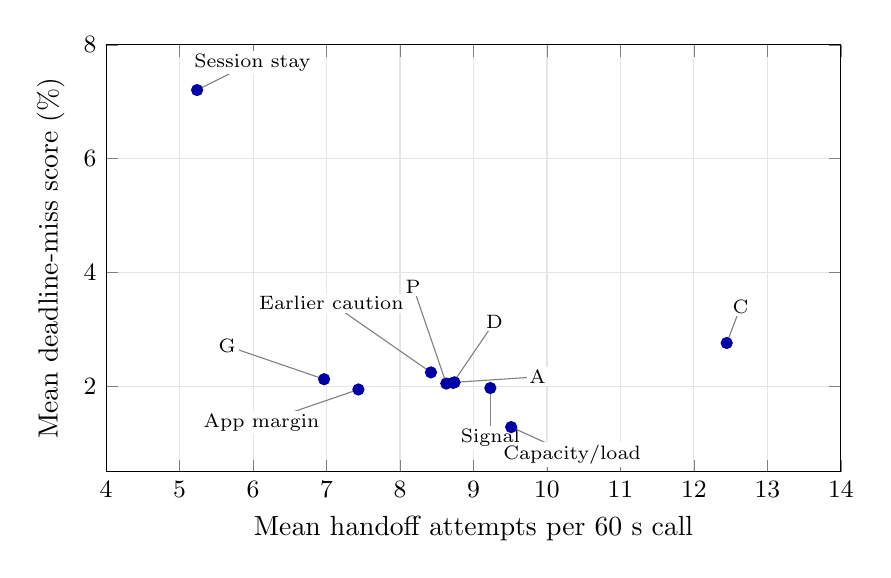
\begin{tikzpicture}\begin{axis}[width=.9\linewidth,height=70mm,
 xlabel={Mean handoff attempts per 60 s call},ylabel={Mean deadline-miss score (\%)},
 xmin=4,xmax=14,ymin=.5,ymax=8,xmajorgrids,ymajorgrids,grid style={gray!20},tick label style={font=\small}]
\addplot[only marks,mark=*,blue!65!black] coordinates {(9.2291667,1.9680093)};
\draw[gray] (axis cs:9.229166666666666,1.9680092592592597) -- ++(0pt,-18pt) node[text=black,fill=white,inner sep=1pt,font=\scriptsize] {Signal};
\addplot[only marks,mark=*,blue!65!black] coordinates {(9.5125,1.2820833)};
\draw[gray] (axis cs:9.5125,1.282083333333334) -- ++(22pt,-10pt) node[text=black,fill=white,inner sep=1pt,font=\scriptsize] {Capacity/load};
\addplot[only marks,mark=*,blue!65!black] coordinates {(7.4333333,1.942662)};
\draw[gray] (axis cs:7.433333333333334,1.942662037037037) -- ++(-35pt,-12pt) node[text=black,fill=white,inner sep=1pt,font=\scriptsize] {App margin};
\addplot[only marks,mark=*,blue!65!black] coordinates {(8.4208333,2.2433333)};
\draw[gray] (axis cs:8.420833333333333,2.2433333333333336) -- ++(-36pt,25pt) node[text=black,fill=white,inner sep=1pt,font=\scriptsize] {Earlier caution};
\addplot[only marks,mark=*,blue!65!black] coordinates {(5.2375,7.2065972)};
\draw[gray] (axis cs:5.2375,7.206597222222221) -- ++(20pt,10pt) node[text=black,fill=white,inner sep=1pt,font=\scriptsize] {Session stay};
\addplot[only marks,mark=*,blue!65!black] coordinates {(8.6291667,2.0470602)};
\draw[gray] (axis cs:8.629166666666666,2.047060185185185) -- ++(-12pt,35pt) node[text=black,fill=white,inner sep=1pt,font=\scriptsize] {P};
\addplot[only marks,mark=*,blue!65!black] coordinates {(8.7208333,2.0593981)};
\draw[gray] (axis cs:8.720833333333333,2.0593981481481483) -- ++(15pt,22pt) node[text=black,fill=white,inner sep=1pt,font=\scriptsize] {D};
\addplot[only marks,mark=*,blue!65!black] coordinates {(6.9666667,2.1231019)};
\draw[gray] (axis cs:6.966666666666667,2.123101851851852) -- ++(-35pt,12pt) node[text=black,fill=white,inner sep=1pt,font=\scriptsize] {G};
\addplot[only marks,mark=*,blue!65!black] coordinates {(12.445833,2.7597454)};
\draw[gray] (axis cs:12.445833333333333,2.7597453703703705) -- ++(5pt,13pt) node[text=black,fill=white,inner sep=1pt,font=\scriptsize] {C};
\addplot[only marks,mark=*,blue!65!black] coordinates {(8.7416667,2.0680324)};
\draw[gray] (axis cs:8.741666666666667,2.0680324074074075) -- ++(30pt,2pt) node[text=black,fill=white,inner sep=1pt,font=\scriptsize] {A};
\end{axis}\end{tikzpicture}
% END GENERATED TRADEOFF
\caption{Mean handoff attempts versus mean deadline-miss score over 240 worlds. Full policy names appear in Table~\ref{tab:main}. Plot abbreviations are P for Proposed, D for No dwell, G for No guard, C for No cost, and A for No age. Closely spaced points represent genuinely similar aggregate values.}\label{fig:tradeoff}
\end{figure}
\FloatBarrier
\begin{thebibliography}{99}
% BEGIN GENERATED BIBLIOGRAPHY
\bibitem{M01} Apple. Wi-Fi roaming support in Apple devices. Official vendor deployment documentation, accessed 14 October 2026.
\url{https://support.apple.com/en-euro/guide/deployment/dep98f116c0f/web}.

\bibitem{F01} Mun-Suk Kim et al. A user application-based access point selection algorithm for dense WLANs. PLOS ONE, 2019.
\url{https://journals.plos.org/plosone/article?id=10.1371/journal.pone.0210738}.

\bibitem{F02} Peter Dely et al. Optimization of WLAN associations considering handover costs. EURASIP Journal on Wireless Communications and Networking, 2012.
\url{https://link.springer.com/article/10.1186/1687-1499-2012-255}.

\bibitem{F03} Toni Adame et al. Channel load aware AP / Extender selection in Home WiFi networks using IEEE 802.11k/v. IEEE Access, 2021.
\url{https://arxiv.org/abs/2004.08110}.

\bibitem{R03} Derrick Qin Sheng Wong, Chong Eng Tan. Enhanced Load-Aware Handover Algorithm for High-Density IEEE 802.11 ESS Networks. ECTI Transactions on Computer and Information Technology, 2025.
\url{https://ph01.tci-thaijo.org/index.php/ecticit/article/view/263263}.

\bibitem{R06} Ting-Hui Wang, Li-Hsiang Shen, Kai-Ten Feng. Distributed Multi-Agent Deep Q-Learning for Fast Roaming in IEEE 802.11ax Wi-Fi Systems. Author preprint, 2023. Later CCNC 2024 version.
\url{https://arxiv.org/abs/2304.01210}.

\bibitem{R04} Ju-Hyung Lee, Yanqing Lu, Klaus Doppler. On-Device LLM for Context-Aware Wi-Fi Roaming. Author preprint, 2025. ML4Wireless 2025 workshop, not ICML main track.
\url{https://arxiv.org/abs/2505.04174}.

\bibitem{R13} Yonghan Kwon, Jae Hong Shin, Jeongyeup Paek. Proactive Roaming Prediction using LSTM in Industrial Wi-Fi-based AGV Networks. 2026 International Conference on Information Networking (ICOIN), 2026.
\url{https://nsl.cau.ac.kr/papers/ictc/icoin2026-kwon-roaming.pdf}.

\bibitem{R07} Stefano Scanzio et al. Multi-Link Operation and Wireless Digital Twin to Support Enhanced Roaming in Next-Gen Wi-Fi. Author preprint, 2024.
\url{https://arxiv.org/abs/2404.18313}.

\bibitem{M06} Pablo Avila-Campos et al. Unlocking Mobility for Wi-Fi-Based Wireless Time-Sensitive Networks. IEEE Access, 2024.
\url{https://doi.org/10.1109/ACCESS.2024.3369481}.

\bibitem{R01} Yoshiko Sueda, Hayato Saiki, Arata Koike. A User-Centric Approach for Controlling Wi-Fi Handover Based on Application Context. IEICE Technical Report, 2026. Abstract/metadata reviewed; full methods not inspected.
\url{https://ken.ieice.org/ken/paper/202603059csa/eng/}.

\bibitem{R02} Adnan Nadeem et al. QoS-Aware Handoff Framework for Performance Optimization in Software-Defined Wi-Fi Networks. Telecommunication Systems, 2026. Abstract/metadata reviewed; full methods not inspected.
\url{https://link.springer.com/article/10.1007/s11235-026-01410-6}.

\bibitem{P01} Randell Jesup, Zaheduzzaman Sarker. Congestion Control Requirements for Interactive Real-Time Media. RFC 8836, 2021.
\url{https://www.rfc-editor.org/rfc/rfc8836.html}.

\bibitem{P02} Julian Spittka, Koen Vos, Jean-Marc Valin. RTP Payload Format for the Opus Speech and Audio Codec. RFC 7587, 2015.
\url{https://www.rfc-editor.org/rfc/rfc7587.html}.

\bibitem{M12} W3C Web Real-Time Communications Working Group. Identifiers for WebRTC's Statistics API. W3C Candidate Recommendation Draft, 2025. Dated 25 September 2025.
\url{https://www.w3.org/TR/2025/CRD-webrtc-stats-20250925/}.

\bibitem{P06} IEEE Author Center. Research Reproducibility. Official publisher reproducibility guidance, accessed 14 October 2026.
\url{https://journals.ieeeauthorcenter.ieee.org/create-your-ieee-journal-article/research-reproducibility/}.

\bibitem{P07} IEEE Author Center. Submission Policies. Official publisher policy, accessed 14 October 2026.
\url{https://conferences.ieeeauthorcenter.ieee.org/author-ethics/guidelines-and-policies/submission-policies/}.
% END GENERATED BIBLIOGRAPHY
\end{thebibliography}
\end{document}
